% LaTEX source code
% Last modified November 1st, 2005
% Steve Miller
% note that the percent sign comments out the rest of the line
% first, we set a document class. often use 12pt characters, though
% sometimes people do 11 or 10. you can do report or article, both similar
%\documentclass[12pt,letterpaper]{article}
\documentclass[12pt,reqno]{amsart}
\linespread{1}
\addtolength{\textwidth}{2cm} \addtolength{\hoffset}{-1cm}
\addtolength{\marginparwidth}{-1cm} \addtolength{\textheight}{2cm}
\addtolength{\voffset}{-1cm}
% below are some packages that are needed for certain symbols, graphics, colors.
% safest to just include these.
\usepackage{times}
\usepackage[T1]{fontenc}
\usepackage{mathrsfs}
\usepackage{latexsym}
\usepackage[dvips]{graphics}
\usepackage{epsfig}
\usepackage{hyperref, amsmath, amsthm, amsfonts, amscd, flafter,epsf}
\usepackage{amsmath,amsfonts,amsthm,amssymb,amscd}
\input amssym.def
\input amssym.tex
\usepackage{color}
\usepackage{enumerate}
\usepackage{hyperref}
\usepackage{url}
\usepackage{floatrow}
\usepackage{caption}
\usepackage{subcaption}
\usepackage{capt-of}
\usepackage{physics}
\newcommand{\todo}[1]{\textcolor{red}{\textbf{(#1)}}}

    %=======================================================

    %   THIS IS WHERE YOU PUT SHORTCUT DEFINITIONS

    %========================================================

% Note that we use a percent sign to comment out a line

% below are shortcut commands

%%%%%%%%%%%%%%%%%%%%%%%%%%%%%%%%%%%%%%%%%%%%%%%

% below are shortcuts for equation, eqnarray,

% itemize and enumerate environments

\newcommand\be{\begin{equation}}
\newcommand\ee{\end{equation}}
\newcommand\bea{\begin{eqnarray}}
\newcommand\eea{\end{eqnarray}}
\newcommand\bi{\begin{itemize}}
\newcommand\ei{\end{itemize}}
\newcommand\ben{\begin{enumerate}}
\newcommand\een{\end{enumerate}}
\newcommand{\ncr}[2]{\left({#1 \atop #2}\right)}
%%%%%%%%%%%%%%%%%%%%%%%%%%%%%%%%%%%%%%%%%%%%%%%%

% Theorem / Lemmas et cetera

\newtheorem{thm}{Theorem}[section]
\newtheorem{conj}[thm]{Conjecture}
\newtheorem{cor}[thm]{Corollary}
\newtheorem{lem}[thm]{Lemma}
\newtheorem{prop}[thm]{Proposition}
\newtheorem{exa}[thm]{Example}
\newtheorem{defi}[thm]{Definition}
\newtheorem{exe}[thm]{Exercise}
\newtheorem{rek}[thm]{Remark}
\newtheorem{que}[thm]{Question}
\newtheorem{prob}[thm]{Problem}
\newtheorem{cla}[thm]{Claim}
\newtheorem{defis}[thm]{Definitions}
\newtheorem{res}[thm]{Result}
\newtheorem{calc}[thm]{Calculation}
%%%%%%%%%%%%%%%%%%%%%%%%%%%%%%%%%%%%%%%%%

% shortcuts to environments

% this allows you to do textboldface: simply type \tbf{what you want in bold}

\newcommand{\tbf}[1]{\textbf{#1}}

%%%%%%%%%%%%%%%%%%%%%%%%%%%%%%%%%%%%%%%%%%%%%%%%%%

% shortcut to twocase and threecase definitions

\newcommand{\twocase}[5]{#1 \begin{cases} #2 & \text{#3}\\ #4
&\text{#5} \end{cases}   }
\newcommand{\threecase}[7]{#1 \begin{cases} #2 &
\text{#3}\\ #4 &\text{#5}\\ #6 &\text{#7} \end{cases}   }
%%%%%%%%%%%%%%%%%%%%%%%%%%%%%%%%%%%%%%%%%

%Blackboard Letters

\newcommand{\R}{\ensuremath{\mathbb{R}}}
\newcommand{\C}{\ensuremath{\mathbb{C}}}
\newcommand{\Z}{\ensuremath{\mathbb{Z}}}
\newcommand{\Q}{\mathbb{Q}}
\newcommand{\N}{\mathbb{N}}
\newcommand{\F}{\mathbb{F}}
\newcommand{\W}{\mathbb{W}}
\newcommand{\Qoft}{\mathbb{Q}(t)}  %use in linux
\newcommand{\soln}{\noindent \textbf{Solution:}\ }

%%%%%%%%%%%%%%%%%%%%%%%%%%%%%%%%%%%%%%%%%

% Finite Fields and Groups

\newcommand{\Fp}{ \F_p }
%%%%%%%%%%%%%%%%%%%%%%%%%%%%%%%%%%%%%%%%%

% Fractions

\newcommand{\foh}{\frac{1}{2}}  %onehalf
\newcommand{\fot}{\frac{1}{3}}
\newcommand{\fof}{\frac{1}{4}}

%%%%%%%%%%%%%%%%%%%%%%%%%%%%%%%%%%%%%%%%%

% Legendre Symbols

\newcommand{\js}[1]{ { \underline{#1} \choose p} }

%%%%%%%%%%%%%%%%%%%%%%%%%%%%%%%%%%%%%%%%%

% matrix shortcuts

\newcommand{\mattwo}[4]
{\left(\begin{array}{cc}
                        #1  & #2   \\
                        #3 &  #4
                          \end{array}\right) }
\newcommand{\matthree}[9]
{\left(\begin{array}{ccc}
                        #1  & #2 & #3  \\
                        #4 &  #5 & #6 \\
                        #7 &  #8 & #9
                          \end{array}\right) }
\newcommand{\dettwo}[4]
{\left|\begin{array}{cc}
                        #1  & #2   \\
                        #3 &  #4
                          \end{array}\right| }
\newcommand{\detthree}[9]
{\left|\begin{array}{ccc}
                        #1  & #2 & #3  \\
                        #4 &  #5 & #6 \\
                        #7 &  #8 & #9
                          \end{array}\right| }
%%%%%%%%%%%%%%%%%%%%%%%%%%%%%%%%%%%%%%%%%

% greek letter shortcuts

\newcommand{\ga}{\alpha}                  %gives you a greek alpha
\newcommand{\gb}{\beta}
\newcommand{\gep}{\epsilon}
%%%%%%%%%%%%%%%%%%%%%%%%%%%%%%%%%%%%%%%%%

% general functions

\newcommand{\notdiv}{\nmid}               % gives the not divide symbol
\newcommand{\burl}[1]{\textcolor{blue}{\url{#1}}}

%%%%%%%%%%%%%%%%%%%%%%%%%%%%%%%%%%%%%%%%%%%

% the following makes the numbering start with 1 in each section;

% if you want the equations numbered 1 to N (without caring about

% what section you are in, comment out the following line.

\numberwithin{equation}{section}

%\textwidth= 6in

%\evensidemargin=37pt

%\oddsidemargin=0pt

\begin{document}



\title{Machine Learning Glasses Results Log}
\author{Kirk Swanson}
\email{swansonk1@uchicago.edu}
\address{Institute for Molecular Engineering, University of Chicago, 5640 S Ellis Ave, Chicago, IL 60637}
%\keywords{path integral molecular dynamics, path integral monte carlo, metropolis algorithm}
\date{\today}




\maketitle

%%%%%%%%%%%%%%%%%%%%%%%%%%%%%%%%%%%%%%%%%%%%%%%%%%%%%%%%%%%%%%%%%%%%%%%%%%%%%%%%%%%%%%%%%%%%%%%%%%%%%%%%%%%%%%%%%%%%%%%%%%%%%%

\normalsize

%%%%%%%%%%%%%%%%%%%%%%%%%%%%%%%%%%%%%%%%%%%%%%%%%%%%%%%%%%%%%%%%%%%%%%%%%%%%%%%%%%%%%%%%%%%%%%%%%%%%%%%%%%%%%%%%%%%%%%%%%%%%%%

%%%%%%%%%%%%%%%%%%%%%%%%%%%%%%%%%%%%%%%%%%%%%%%%%%%%%%%%%%%%%%%%%%%%%%%%%%%%%%%%%%%%%%%%%%%%%%%%%%%%%%%%%%%%%%%%%%%%%%%%%%%%%%

\section{11/26/2017}
\begin{enumerate}
\item Merged recent updates to GitHub
\item Downloaded images from a while ago.  This first one is batch size 80, learning rate 0.001, beta 0.01, dropout 0.5, including the recent change that each batch is chosen from a newly randomly chuffled metadata:
\begin{figure}[H]
\centering
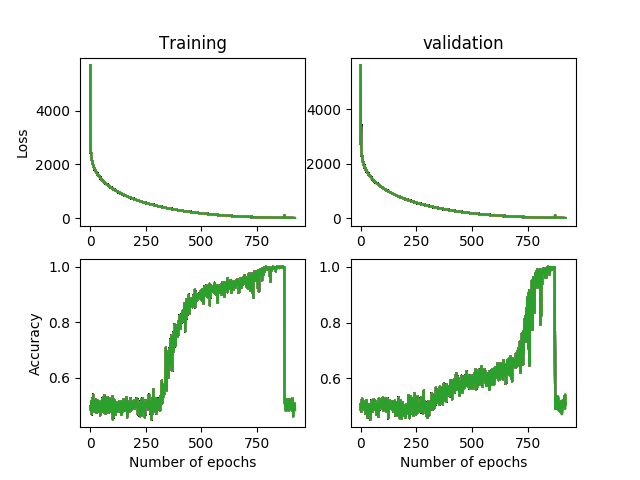
\includegraphics[scale=0.6]{test-batch2-1e-3-80-1e-2-5e-1}
\caption{Batch Size = 80, Learning Rate = 1e-3, Beta = 0.01, Dropout = 0.5}
\end{figure}
\item This run had an optimal validation accuracy of 99.7635 and an optimal test accuracy of 99.7297.  I also tested this multiple times, running the SAME set of hyperparameters, to see what is going on with that weird spike.  Does it keep showing up?  What is going on?  Here are more examples, all run at the same hyperparameters as above:
\begin{figure}[H]
\centering
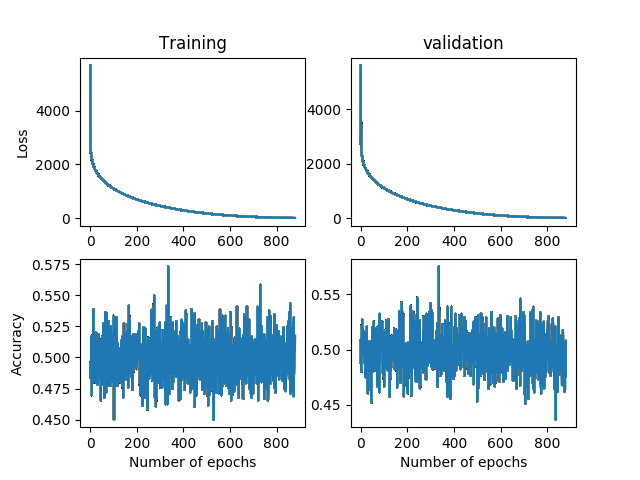
\includegraphics[scale=0.6]{learning-rate-rep1-1e-3-80-1e-2-5e-1}
\caption{Batch Size = 80, Learning Rate = 1e-3, Beta = 0.01, Dropout = 0.5}
\end{figure}
\item This run had an optimal validation accuracy of 47.0608, optimal test accuracy of 47.6689, and final validation accuracy of 49.223, test accuracy of 50.0338 

\begin{figure}[H]
\centering
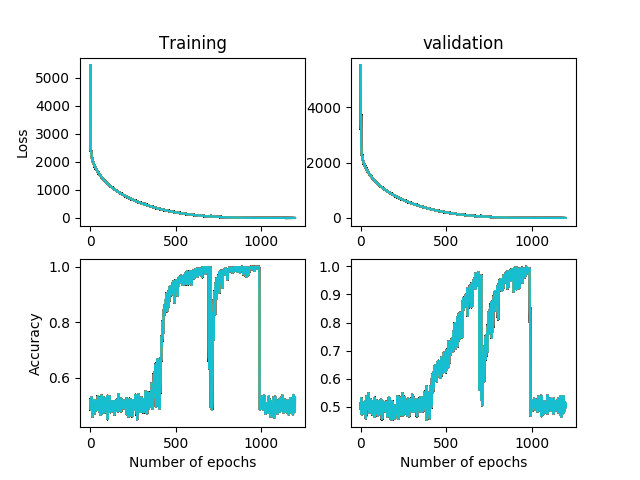
\includegraphics[scale=0.6]{learning-rate-rep2-1e-3-80-1e-2-5e-1}
\caption{Batch Size = 80, Learning Rate = 1e-3, Beta = 0.01, Dropout = 0.5}
\end{figure}
\item This run had an optimal validation accuracy of 99.4595, optimal test accuracy of 99.3243, and final validation accuracy of 50.777, test accuracy of 49.9662. 

\begin{figure}[H]
\centering
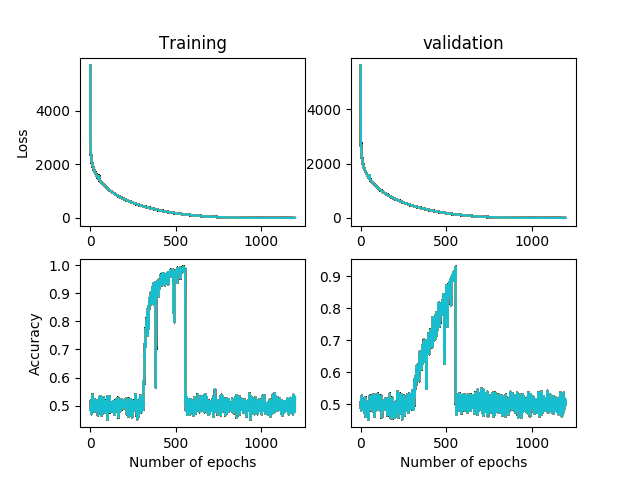
\includegraphics[scale=0.6]{learning-rate-rep3-1e-3-80-1e-2-5e-1}
\caption{Batch Size = 80, Learning Rate = 1e-3, Beta = 0.01, Dropout = 0.5}
\end{figure}
\item This run had an optimal validation accuracy of 992.5, optimal test accuracy of 91.7568, and final validation accuracy of 49.223, test accuracy of 50.0338. 

\begin{figure}[H]
\centering
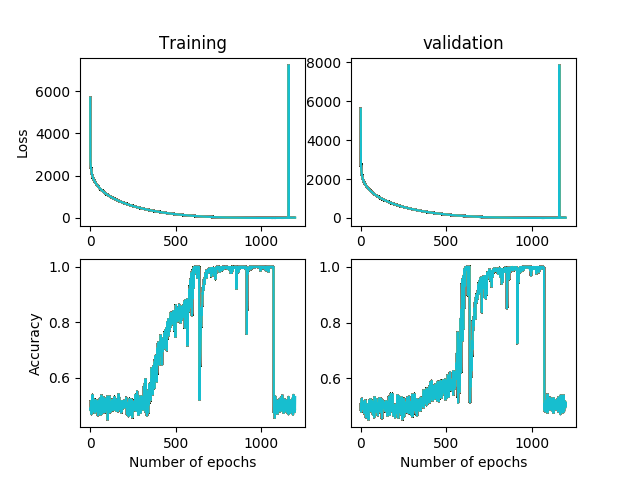
\includegraphics[scale=0.6]{learning-rate-rep4-1e-3-80-1e-2-5e-1}
\caption{Batch Size = 80, Learning Rate = 1e-3, Beta = 0.01, Dropout = 0.5}
\end{figure}
\item This run had an optimal validation accuracy of 99.8987, optimal test accuracy of 99.8649, and final validation accuracy of 50.777, test accuracy of 49.9662. 

\begin{figure}[H]
\centering
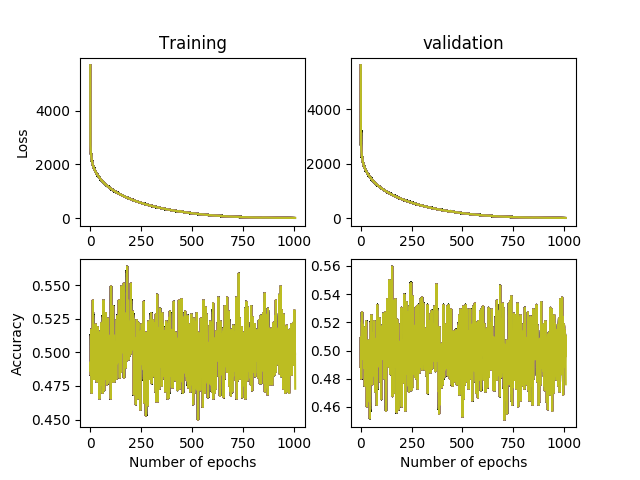
\includegraphics[scale=0.6]{learning-rate-rep5-1e-3-80-1e-2-5e-1}
\caption{Batch Size = 80, Learning Rate = 1e-3, Beta = 0.01, Dropout = 0.5}
\end{figure}
\item This run had an optimal validation accuracy of 55.4054, optimal test accuracy of 54.223, and final validation accuracy of 49,223, test accuracy of 50.0338.

\item The following are images of runs on the dataset that consists of glasses and liquids that are each 12 time steps away from the assumed glass transition temperature of 0.21.  

\begin{figure}[H]
\centering
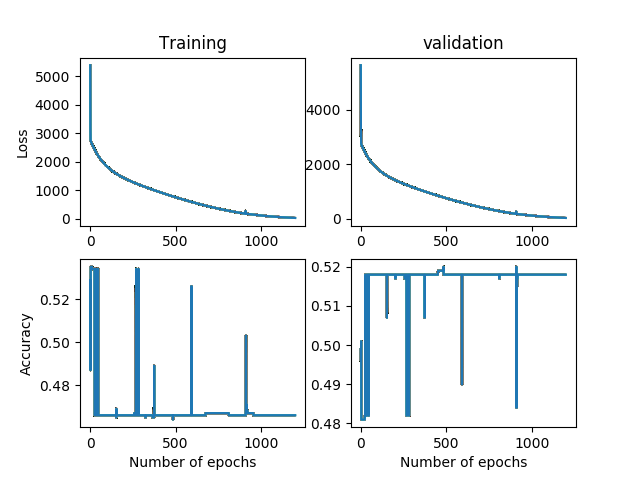
\includegraphics[scale=0.6]{data12-1e-4-100-1e-2-5e-1}
\caption{Batch Size = 100, Learning Rate = 1e-4, Beta = 0.01, Dropout = 0.5}
\end{figure}

\begin{figure}[H]
\centering
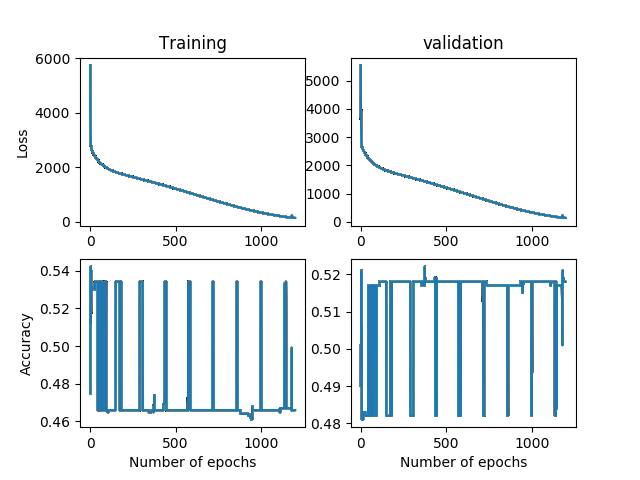
\includegraphics[scale=0.6]{data12-1e-4-10-1e-2-5e-1}
\caption{Batch Size = 10, Learning Rate = 1e-4, Beta = 0.01, Dropout = 0.5}
\end{figure}

\begin{figure}[H]
\centering
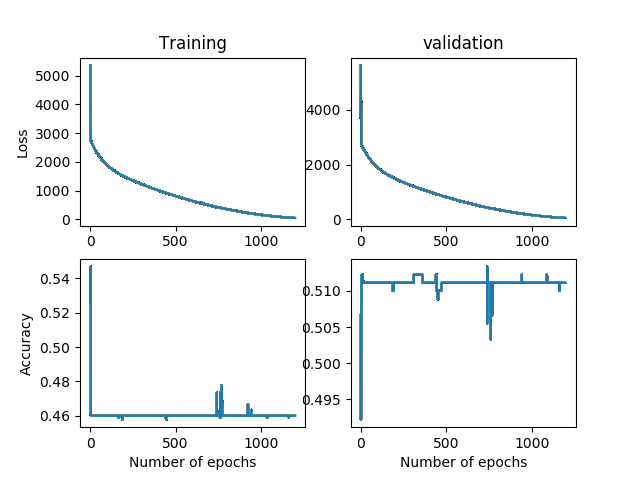
\includegraphics[scale=0.6]{data12-1e-4-150-1e-2-5e-1}
\caption{Batch Size = 150, Learning Rate = 1e-4, Beta = 0.01, Dropout = 0.5}
\end{figure}

\begin{figure}[H]
\centering
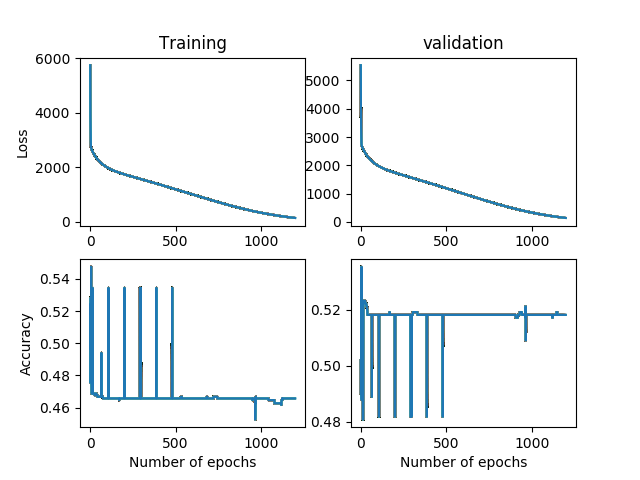
\includegraphics[scale=0.6]{data12-1e-4-15-1e-2-5e-1}
\caption{Batch Size = 15, Learning Rate = 1e-4, Beta = 0.01, Dropout = 0.5}
\end{figure}

\begin{figure}[H]
\centering
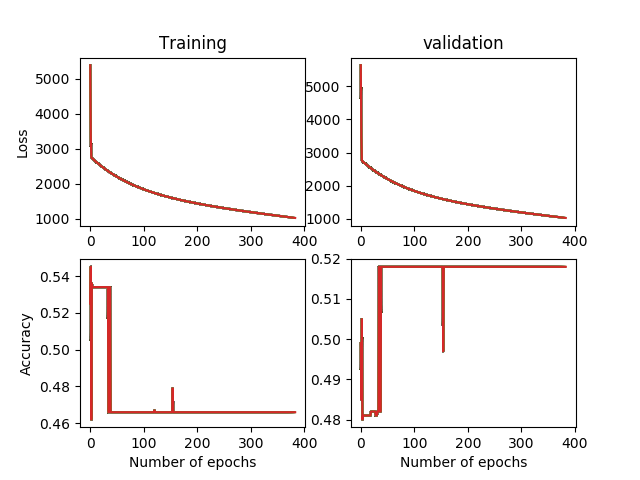
\includegraphics[scale=0.6]{data12-1e-4-200-1e-2-5e-1}
\caption{Batch Size = 200, Learning Rate = 1e-4, Beta = 0.01, Dropout = 0.5}
\end{figure}

\begin{figure}[H]
\centering
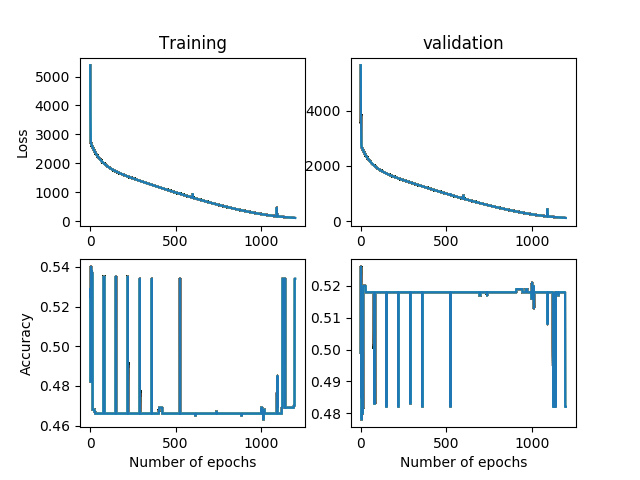
\includegraphics[scale=0.6]{data12-1e-4-20-1e-2-5e-1}
\caption{Batch Size = 20, Learning Rate = 1e-4, Beta = 0.01, Dropout = 0.5}
\end{figure}

\begin{figure}[H]
\centering
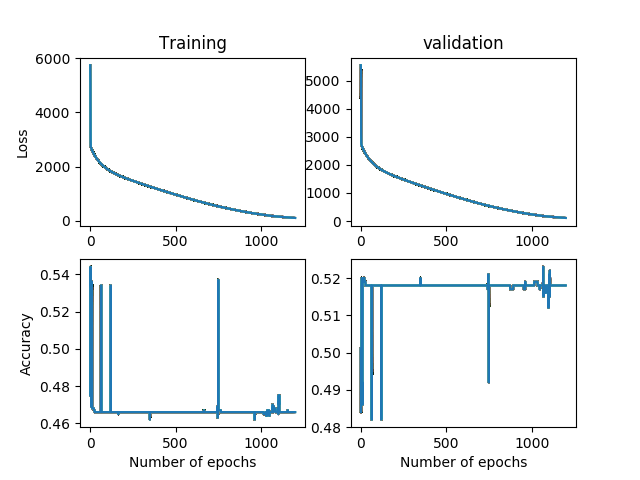
\includegraphics[scale=0.6]{data12-1e-4-25-1e-2-5e-1}
\caption{Batch Size = 25, Learning Rate = 1e-4, Beta = 0.01, Dropout = 0.5}
\end{figure}

\begin{figure}[H]
\centering
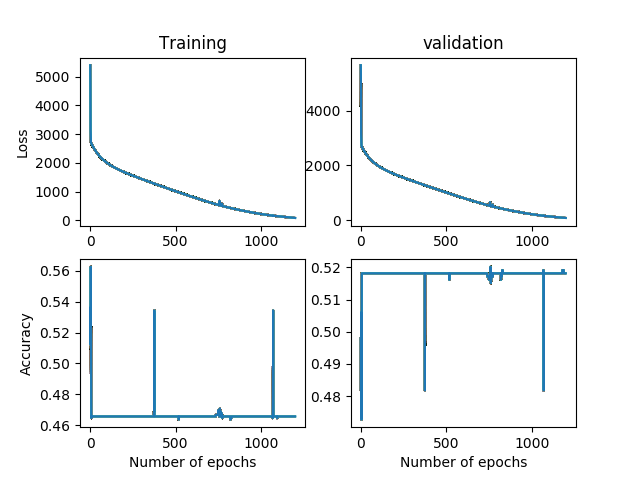
\includegraphics[scale=0.6]{data12-1e-4-30-1e-2-5e-1}
\caption{Batch Size = 30, Learning Rate = 1e-4, Beta = 0.01, Dropout = 0.5}
\end{figure}

\begin{figure}[H]
\centering
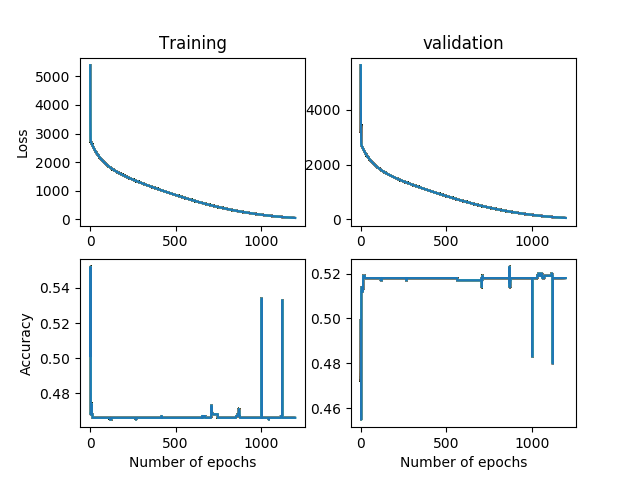
\includegraphics[scale=0.6]{data12-1e-4-50-1e-2-5e-1}
\caption{Batch Size = 50, Learning Rate = 1e-4, Beta = 0.01, Dropout = 0.5}
\end{figure}

\begin{figure}[H]
\centering
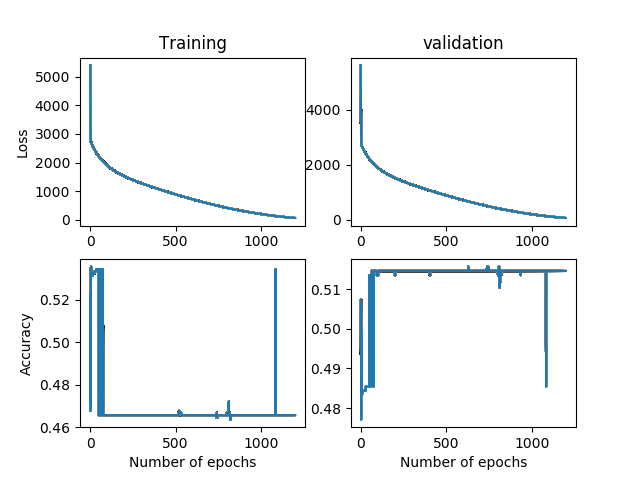
\includegraphics[scale=0.6]{data12-1e-4-80-1e-2-5e-1}
\caption{Batch Size = 80, Learning Rate = 1e-4, Beta = 0.01, Dropout = 0.5}
\end{figure}

\begin{figure}[H]
\centering
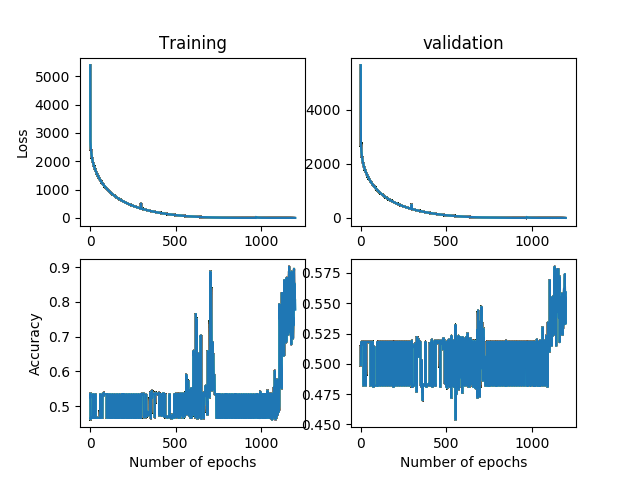
\includegraphics[scale=0.6]{data12-1e-3-100-1e-2-5e-1}
\caption{Batch Size = 100, Learning Rate = 1e-3, Beta = 0.01, Dropout = 0.5}
\end{figure}

\begin{figure}[H]
\centering
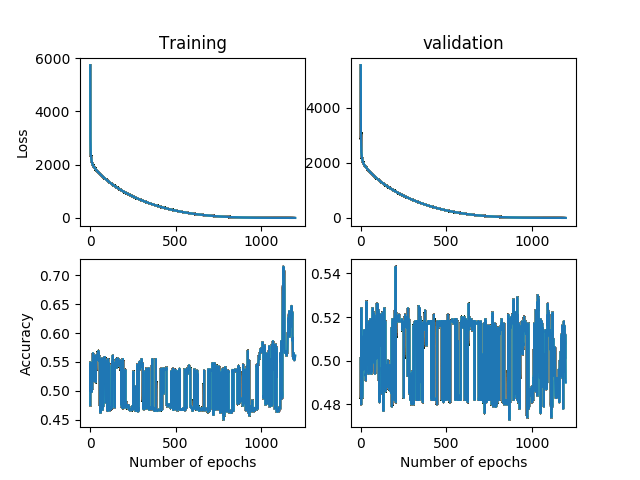
\includegraphics[scale=0.6]{data12-1e-3-10-1e-2-5e-1}
\caption{Batch Size = 10, Learning Rate = 1e-3, Beta = 0.01, Dropout = 0.5}
\end{figure}

\begin{figure}[H]
\centering
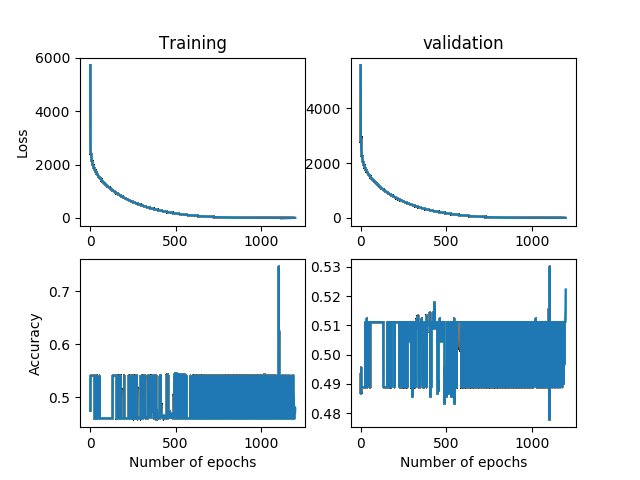
\includegraphics[scale=0.6]{data12-1e-3-150-1e-2-5e-1}
\caption{Batch Size = 150, Learning Rate = 1e-3, Beta = 0.01, Dropout = 0.5}
\end{figure}

\begin{figure}[H]
\centering
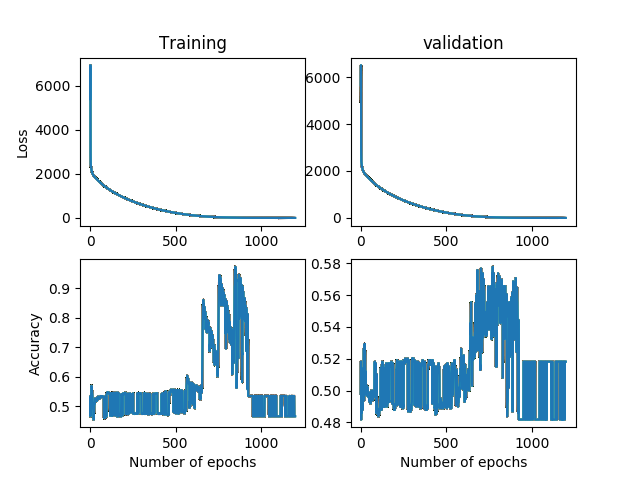
\includegraphics[scale=0.6]{data12-1e-3-15-1e-2-5e-1}
\caption{Batch Size = 15, Learning Rate = 1e-3, Beta = 0.01, Dropout = 0.5}
\end{figure}

\begin{figure}[H]
\centering
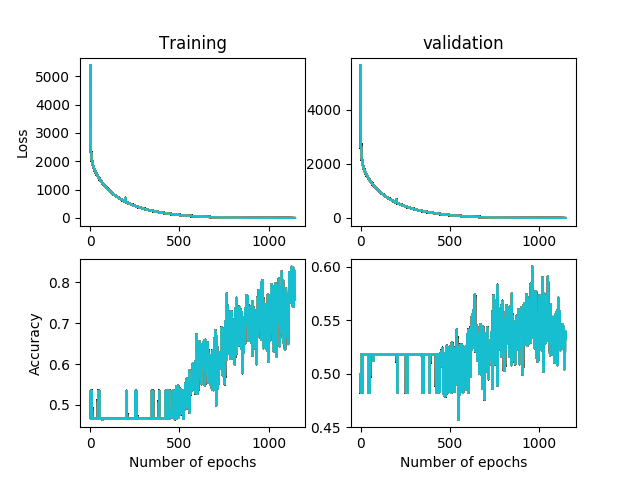
\includegraphics[scale=0.6]{data12-1e-3-200-1e-2-1e-1}
\caption{Batch Size = 200, Learning Rate = 1e-3, Beta = 0.01, Dropout = 0.1}
\end{figure}

\begin{figure}[H]
\centering
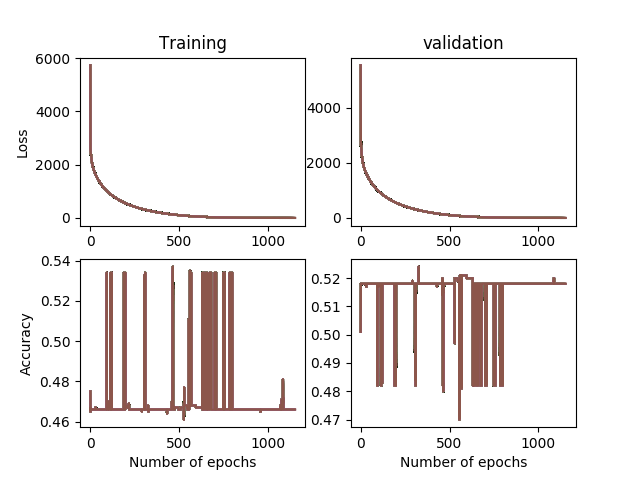
\includegraphics[scale=0.6]{data12-1e-3-200-1e-2-2e-1}
\caption{Batch Size = 200, Learning Rate = 1e-3, Beta = 0.01, Dropout = 0.2}
\end{figure}

\begin{figure}[H]
\centering
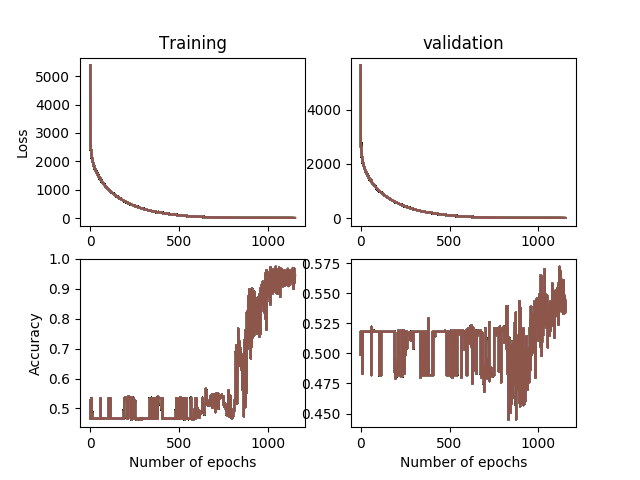
\includegraphics[scale=0.6]{data12-1e-3-200-1e-2-3e-1}
\caption{Batch Size = 200, Learning Rate = 1e-3, Beta = 0.01, Dropout = 0.3}
\end{figure}

\begin{figure}[H]
\centering
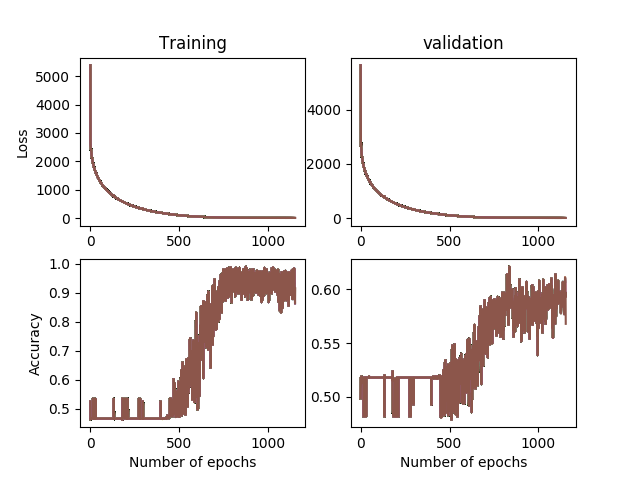
\includegraphics[scale=0.6]{data12-1e-3-200-1e-2-4e-1}
\caption{Batch Size = 200, Learning Rate = 1e-3, Beta = 0.01, Dropout = 0.4}
\end{figure}

\begin{figure}[H]
\centering
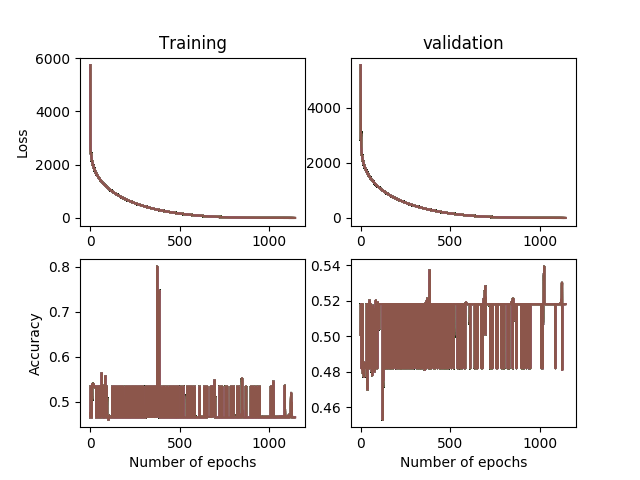
\includegraphics[scale=0.6]{data12-1e-3-200-1e-2-5e-1}
\caption{Batch Size = 200, Learning Rate = 1e-3, Beta = 0.01, Dropout = 0.5}
\end{figure}

\begin{figure}[H]
\centering
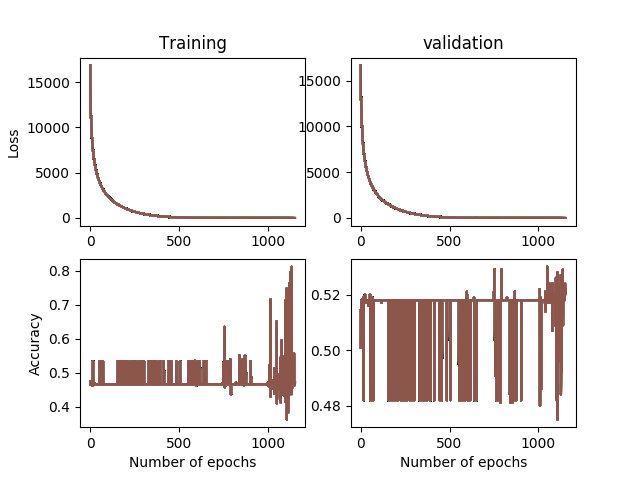
\includegraphics[scale=0.6]{data12-1e-3-200-5e-2-3e-1}
\caption{Batch Size = 200, Learning Rate = 1e-3, Beta = 0.01, Dropout = 0.3}
\end{figure}

\begin{figure}[H]
\centering
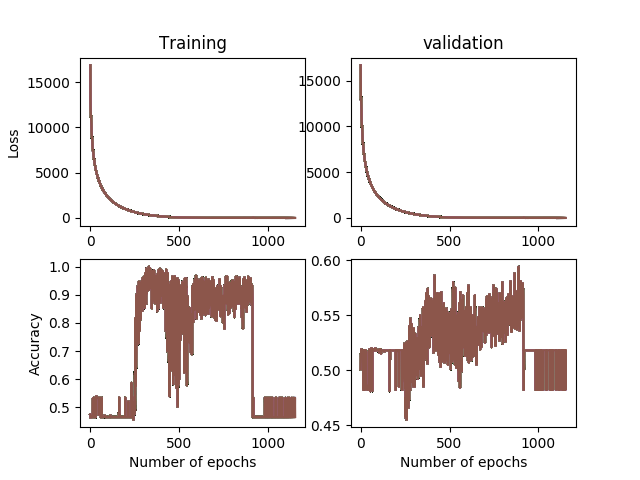
\includegraphics[scale=0.6]{data12-1e-3-200-5e-2-4e-1}
\caption{Batch Size = 200, Learning Rate = 1e-3, Beta = 0.01, Dropout = 0.4}
\end{figure}

\begin{figure}[H]
\centering
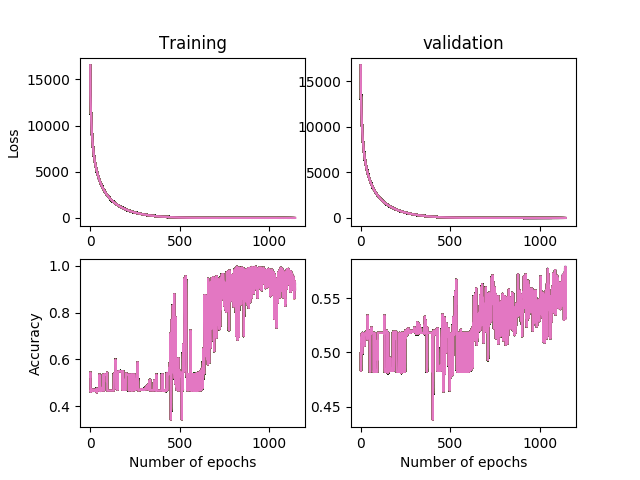
\includegraphics[scale=0.6]{data12-1e-3-200-5e-2-5e-1}
\caption{Batch Size = 200, Learning Rate = 1e-3, Beta = 0.01, Dropout = 0.4}
\end{figure}

\begin{figure}[H]
\centering
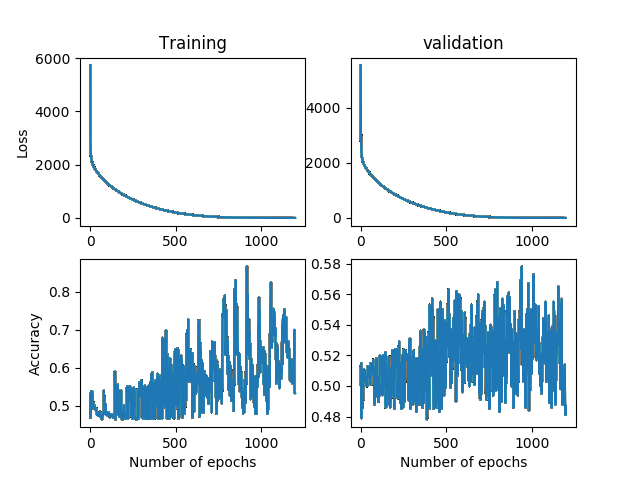
\includegraphics[scale=0.6]{data12-1e-3-20-1e-2-5e-1}
\caption{Batch Size = 20, Learning Rate = 1e-3, Beta = 0.01, Dropout = 0.5}
\end{figure}

\begin{figure}[H]
\centering
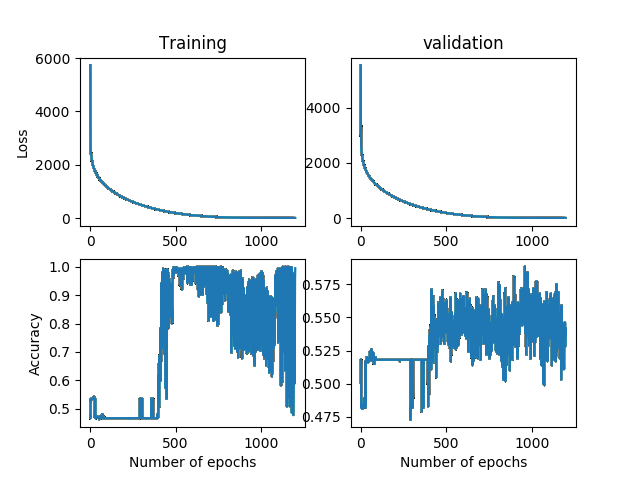
\includegraphics[scale=0.6]{data12-1e-3-250-1e-2-5e-1}
\caption{Batch Size = 250, Learning Rate = 1e-3, Beta = 0.01, Dropout = 0.5}
\end{figure}

\begin{figure}[H]
\centering
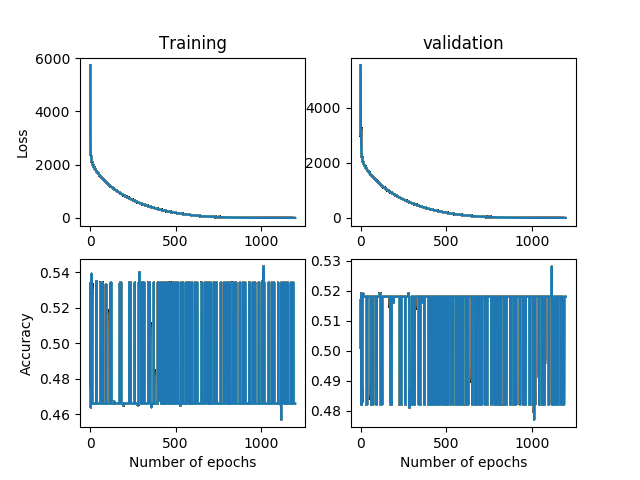
\includegraphics[scale=0.6]{data12-1e-3-25-1e-2-5e-1}
\caption{Batch Size = 25, Learning Rate = 1e-3, Beta = 0.01, Dropout = 0.5}
\end{figure}

\begin{figure}[H]
\centering
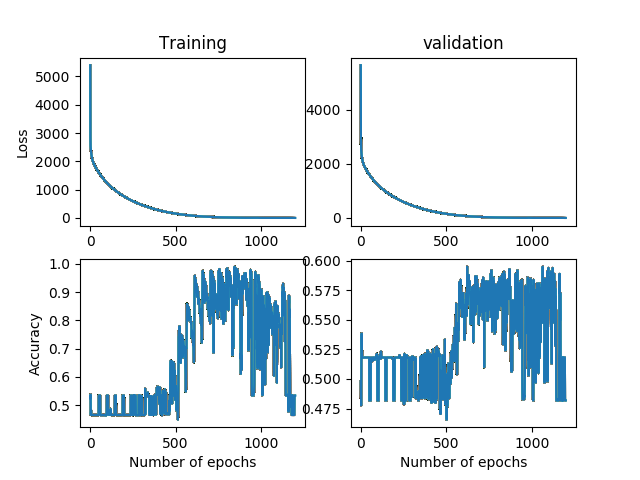
\includegraphics[scale=0.6]{data12-1e-3-30-1e-2-5e-1}
\caption{Batch Size = 30, Learning Rate = 1e-3, Beta = 0.01, Dropout = 0.5}
\end{figure}

\begin{figure}[H]
\centering
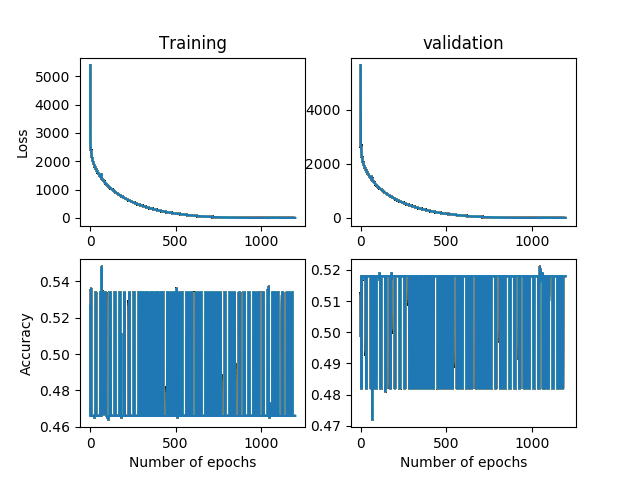
\includegraphics[scale=0.6]{data12-1e-3-50-1e-2-5e-1}
\caption{Batch Size = 50, Learning Rate = 1e-3, Beta = 0.01, Dropout = 0.5}
\end{figure}

\item Visualizations.  
\begin{figure}[H]
\centering
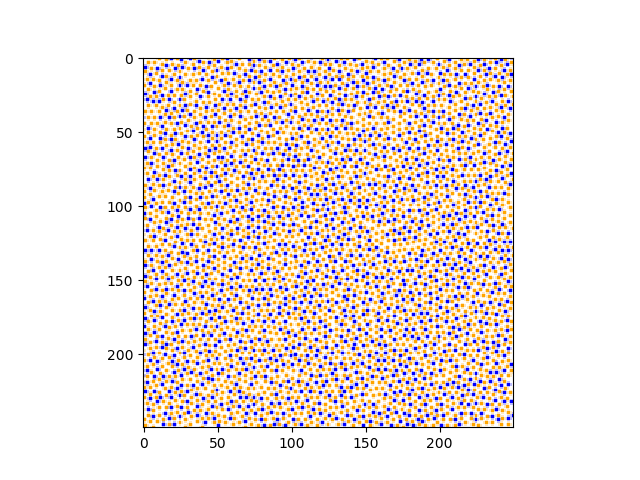
\includegraphics[scale=0.6]{glass_original}
\caption{Glass original}
\end{figure}

\begin{figure}[H]
\centering
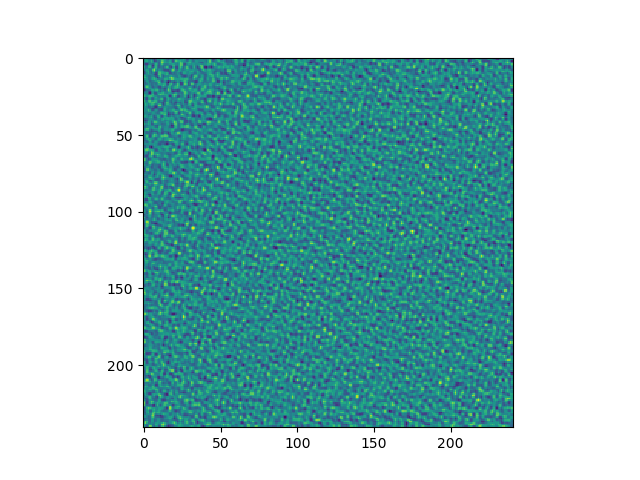
\includegraphics[scale=0.6]{glass_channel_1}
\caption{Glass channel 1}
\end{figure}

\begin{figure}[H]
\centering
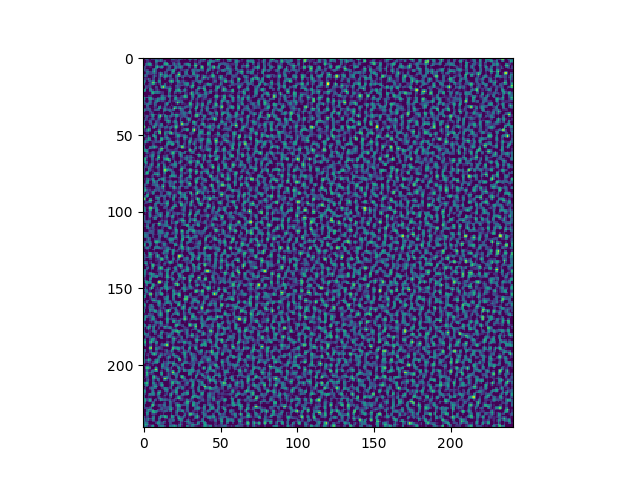
\includegraphics[scale=0.6]{glass_channel_2}
\caption{Glass channel 2}
\end{figure}

\begin{figure}[H]
\centering
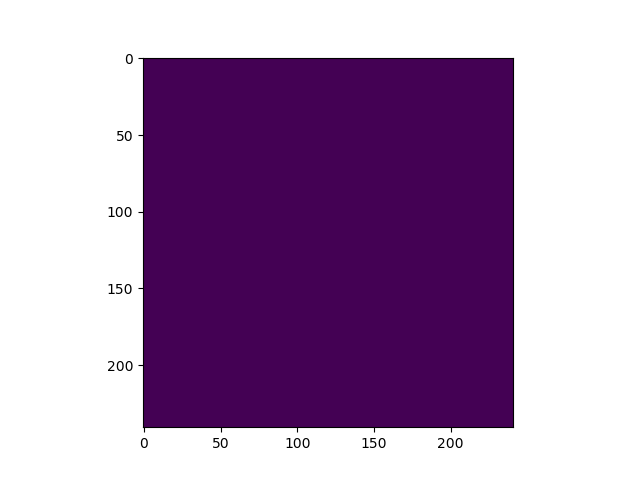
\includegraphics[scale=0.6]{glass_channel_3}
\caption{Glass channel 3}
\end{figure}

\begin{figure}[H]
\centering
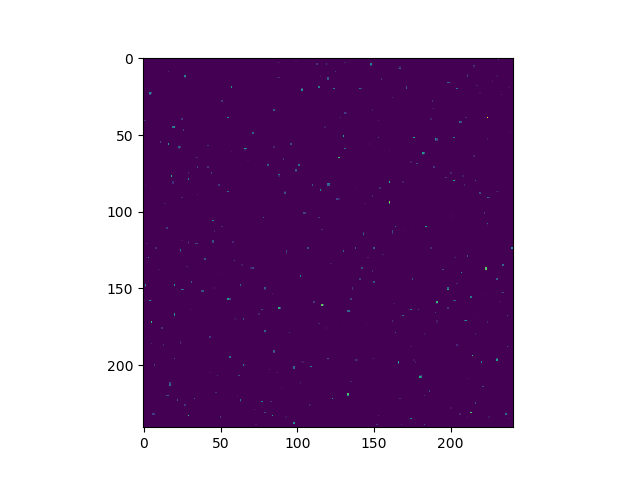
\includegraphics[scale=0.6]{glass_channel_4}
\caption{Glass channel 4}
\end{figure}

\begin{figure}[H]
\centering
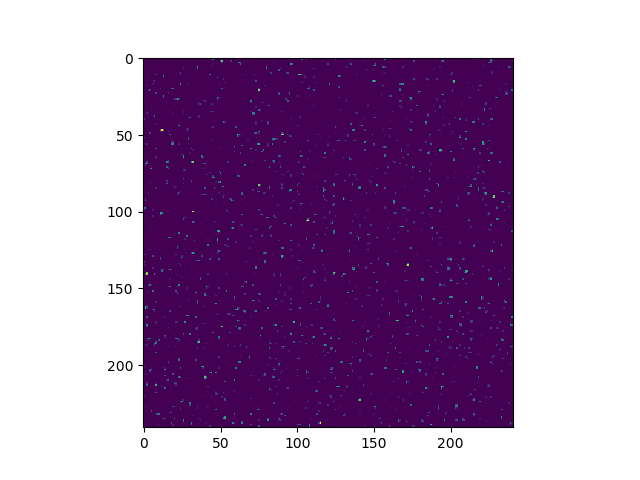
\includegraphics[scale=0.6]{glass_channel_5}
\caption{Glass channel 5}
\end{figure}

\begin{figure}[H]
\centering
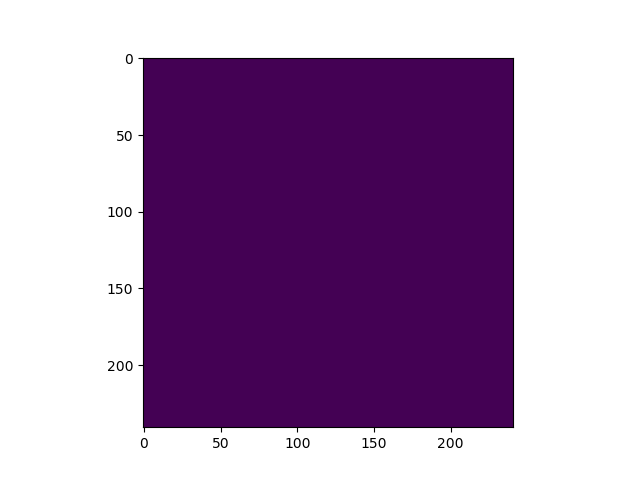
\includegraphics[scale=0.6]{glass_channel_6}
\caption{Glass channel 6}
\end{figure}

\begin{figure}[H]
\centering
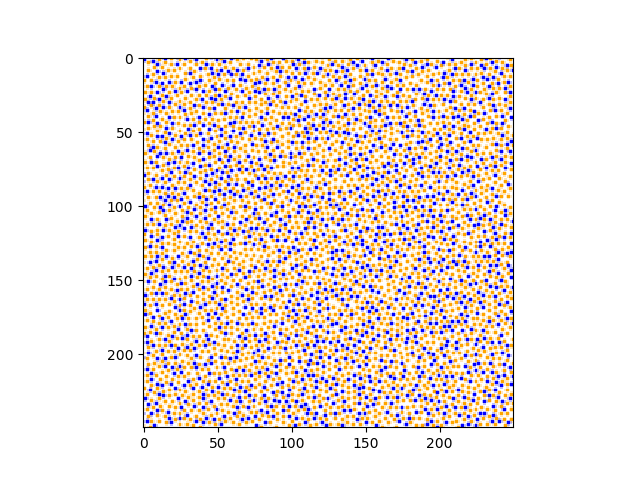
\includegraphics[scale=0.6]{liquid_original}
\caption{Liquid original}
\end{figure}

\begin{figure}[H]
\centering
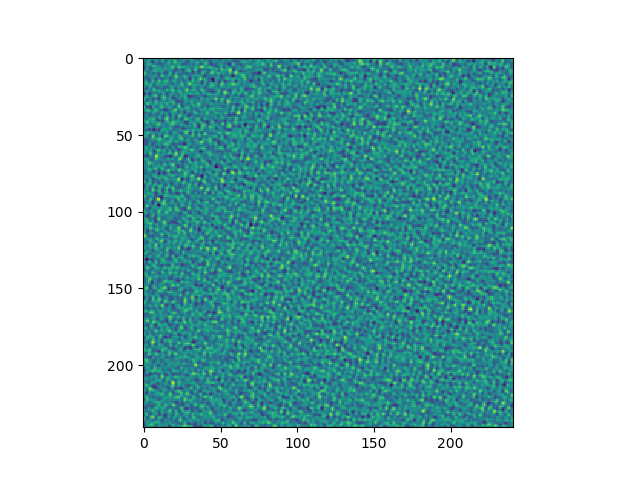
\includegraphics[scale=0.6]{liquid_channel_1}
\caption{Liquid channel 1}
\end{figure}

\begin{figure}[H]
\centering
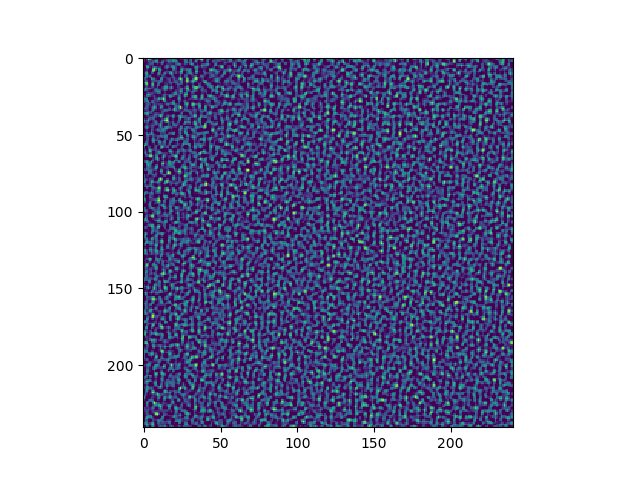
\includegraphics[scale=0.6]{liquid_channel_2}
\caption{Liquid channel 2}
\end{figure}

\begin{figure}[H]
\centering
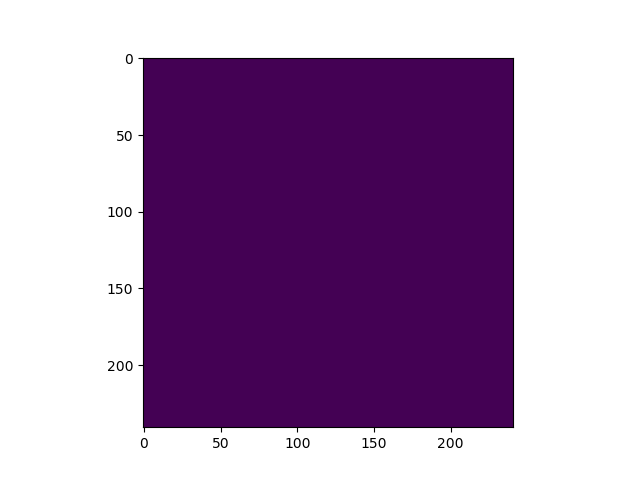
\includegraphics[scale=0.6]{liquid_channel_3}
\caption{Liquid channel 3}
\end{figure}

\begin{figure}[H]
\centering
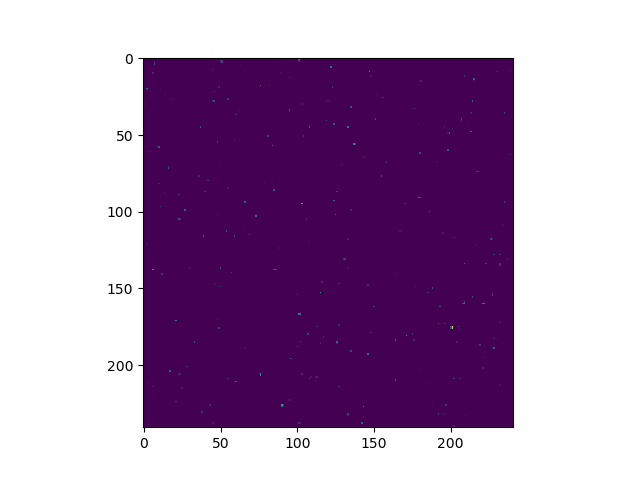
\includegraphics[scale=0.6]{liquid_channel_4}
\caption{Liquid channel 4}
\end{figure}

\begin{figure}[H]
\centering
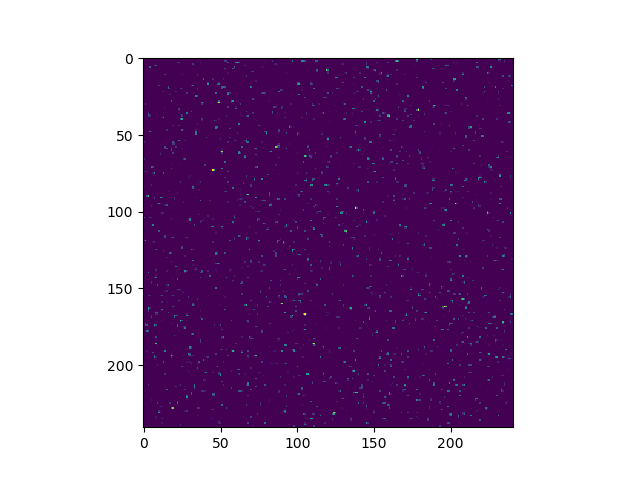
\includegraphics[scale=0.6]{liquid_channel_5}
\caption{Liquid channel 5}
\end{figure}

\begin{figure}[H]
\centering
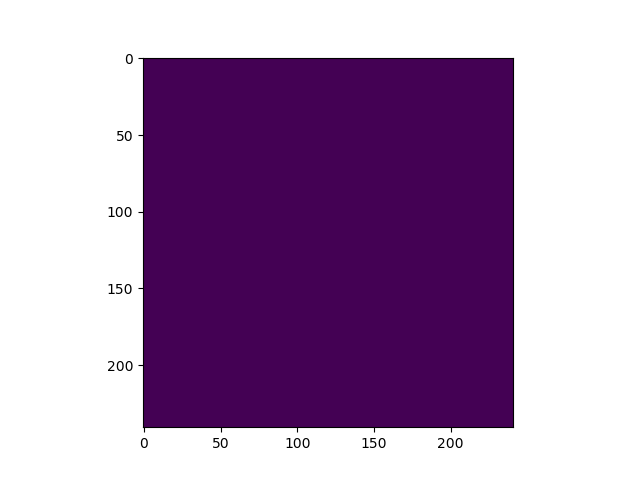
\includegraphics[scale=0.6]{liquid_channel_6}
\caption{Liquid channel 6}
\end{figure}

\end{enumerate}

\section{12/13/2017}
\begin{enumerate}
\item Updated python scripts and merged with GitHub - the recent additions include streamlining the learning rate schedule and data augmentation options.  The following is for a standard run on the original endpoint data:

\begin{figure}[H]
\centering
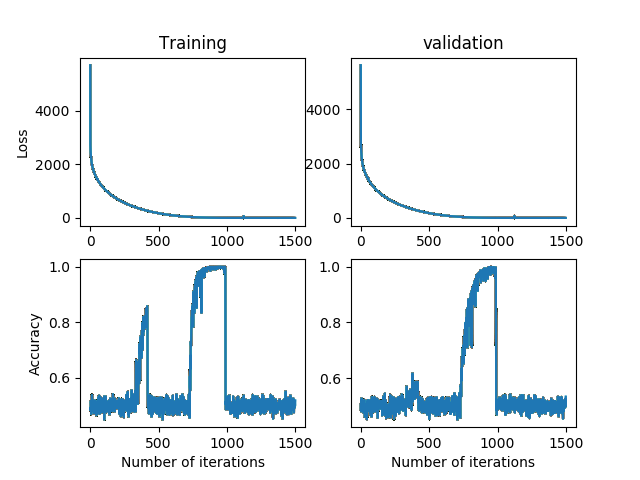
\includegraphics[scale=0.6]{test-1e-3-1e-3-550-80-1e-2-5e-1}
\caption{Initial Learning Rate = 1e-3, Final Learning Rate = 1e-3, Schedule Length = 550 iterations, Batch Size = 80, L2 beta = 0.01, Dropout = 0.5}
\end{figure}

\item I then, twice, set the final learning rate to be smaller, at 1e-4:

\begin{figure}[H]
\centering
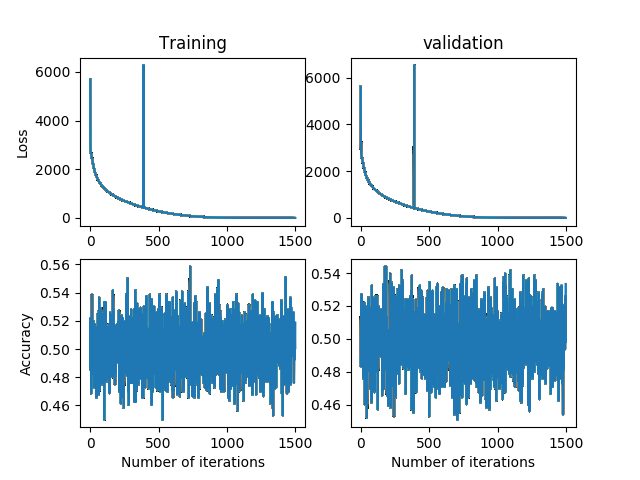
\includegraphics[scale=0.6]{test-1e-4-1e-3-550-80-1e-2-5e-1}
\caption{Initial Learning Rate = 1e-3, Final Learning Rate = 1e-3, Schedule Length = 550 iterations, Batch Size = 80, L2 beta = 0.01, Dropout = 0.5}
\end{figure}

\begin{figure}[H]
\centering
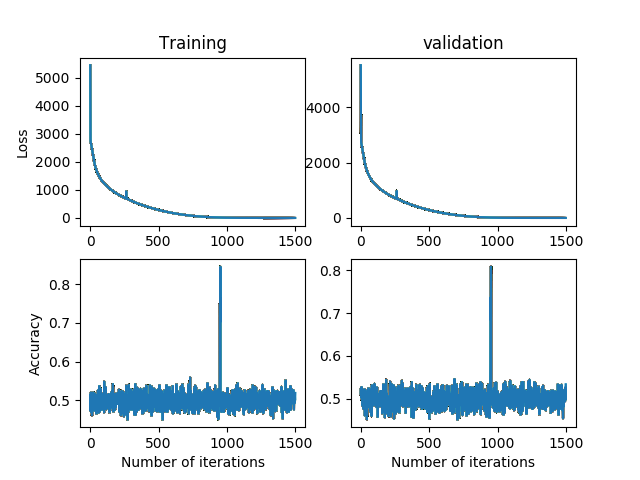
\includegraphics[scale=0.6]{test2-1e-4-1e-3-550-80-1e-2-5e-1}
\caption{Initial Learning Rate = 1e-3, Final Learning Rate = 1e-3, Schedule Length = 550 iterations, Batch Size = 80, L2 beta = 0.01, Dropout = 0.5}
\end{figure}

\item What is going on here?  It seems as though setting the learning rate a magnitude lower really screws things up...
\item Note: one iteration goes through 10 batches, so if the batch size is 80, then one iteration goes through 800 examples.  The training set is 70 percent of the total 20,000 images, so the training set is 14,000 images.  Thus, one epoch is 17.5 iterations, or approximately 18 iterations.  That means that 1500 iterations is about 83 epochs.  Question: how many epochs is typically needed for a binary classification problem?  And how long does this typically take?
\item I also tested the usual hyperparameters on the original endpoint data and turned on the data augmentation, to see if there would be any issues.  I got the following training runs:

\begin{figure}[H]
\centering
\includegraphics[scale=0.6]{data_aug}
\caption{Initial Learning Rate = NA, Final Learning Rate = 1e-3, Schedule Length = NA, Batch Size = 80, L2 beta = 0.01, Dropout = 0.5}
\end{figure}

\begin{figure}[H]
\centering
\includegraphics[scale=0.6]{data_aug2}
\caption{Initial Learning Rate = NA, Final Learning Rate = 1e-3, Schedule Length = NA, Batch Size = 80, L2 beta = 0.01, Dropout = 0.5}
\end{figure}

\begin{figure}[H]
\centering
\includegraphics[scale=0.6]{data_aug3}
\caption{Initial Learning Rate = NA, Final Learning Rate = 1e-3, Schedule Length = NA, Batch Size = 80, L2 beta = 0.01, Dropout = 0.5}
\end{figure}

\begin{figure}[H]
\centering
\includegraphics[scale=0.6]{data_aug4}
\caption{Initial Learning Rate = NA, Final Learning Rate = 1e-3, Schedule Length = NA, Batch Size = 80, L2 beta = 0.01, Dropout = 0.5}
\end{figure}

\begin{figure}[H]
\centering
\includegraphics[scale=0.6]{data_aug5}
\caption{Initial Learning Rate = NA, Final Learning Rate = 1e-3, Schedule Length = NA, Batch Size = 80, L2 beta = 0.01, Dropout = 0.5}
\end{figure}

\item I should double check that the dataset augmentation is actually working.  
\end{enumerate}
\section{12/22/2017}
\begin{enumerate}
\item I am now going to run a series of training runs that will explore the relationship between the learning rate schedule and accuracy.  First, let's try the threshold idea.  Then, we will try the standard exponential decay idea.  Let's try the following.  When the accuracy gets to 90 percent, let's decrease the learning rate by an order of magnitude.  Let's just run that simple test, say, 8 times, and see what happens!

\item Initial learning rate = , Final learning rate = ,   
\end{enumerate}
\section{12/24/2017}
\begin{enumerate}
\item We ran a series of training runs that used a learning rate threshold.  The learning rate starts at the initial learning rate.  The learning rate changes to the final learning rate whenever the validation accuracy is above 90 percent.  This allows the learning rate to go back to the initial learning rate if the accuracy drops below 90 percent.  Here are plots showing six tests.  These plots demonstrate that the sharp drops in accuracy were, indeed, the result of a learning rate that was too large towards the end of training, since there are no sharp drops in accuracy here:

\begin{figure}[H]
\centering
\includegraphics[scale=0.6]{threshold-test-1e-3-1e-4-1}
\caption{Initial Learning Rate = 1e-3, Final Learning Rate = 1e-4, Schedule Length = NA, Batch Size = 80, L2 beta = 0.01, Dropout = 0.5}
\end{figure}

\begin{figure}[H]
\centering
\includegraphics[scale=0.6]{threshold-test-1e-3-1e-4-2}
\caption{Initial Learning Rate = 1e-3, Final Learning Rate = 1e-4, Schedule Length = NA, Batch Size = 80, L2 beta = 0.01, Dropout = 0.5}
\end{figure}

\begin{figure}[H]
\centering
\includegraphics[scale=0.6]{threshold-test-1e-3-1e-4-3}
\caption{Initial Learning Rate = 1e-3, Final Learning Rate = 1e-4, Schedule Length = NA, Batch Size = 80, L2 beta = 0.01, Dropout = 0.5}
\end{figure}

\begin{figure}[H]
\centering
\includegraphics[scale=0.6]{threshold-test-1e-3-1e-5-1}
\caption{Initial Learning Rate = 1e-3, Final Learning Rate = 1e-4, Schedule Length = NA, Batch Size = 80, L2 beta = 0.01, Dropout = 0.5}
\end{figure}

\begin{figure}[H]
\centering
\includegraphics[scale=0.6]{threshold-test-1e-3-1e-5-2}
\caption{Initial Learning Rate = 1e-3, Final Learning Rate = 1e-4, Schedule Length = NA, Batch Size = 80, L2 beta = 0.01, Dropout = 0.5}
\end{figure}

\begin{figure}[H]
\centering
\includegraphics[scale=0.6]{threshold-test-1e-3-1e-5-3}
\caption{Initial Learning Rate = 1e-3, Final Learning Rate = 1e-4, Schedule Length = NA, Batch Size = 80, L2 beta = 0.01, Dropout = 0.5}
\end{figure}

\end{enumerate}

\subsection{12/29/2017}
\begin{enumerate}
\item Ran another series of runs that used a similar learning rate threshold just to check that my GitHub had been updated appropriately.  This time used only 1e-3 to 1e-4.  In one example, the accuracy crashed.  Perhaps evidences that smaller learning rates are needed closer to the minimum.  For the sake of completeness, these extra runs are reported below:  

\begin{figure}[H]
\centering
\includegraphics[scale=0.6]{Commit-test-1}
\caption{Initial Learning Rate = 1e-3, Final Learning Rate = 1e-4, Schedule Length = NA, Batch Size = 80, L2 beta = 0.01, Dropout = 0.5}
\end{figure}

\begin{figure}[H]
\centering
\includegraphics[scale=0.6]{Commit-test-2}
\caption{Initial Learning Rate = 1e-3, Final Learning Rate = 1e-4, Schedule Length = NA, Batch Size = 80, L2 beta = 0.01, Dropout = 0.5}
\end{figure}

\begin{figure}[H]
\centering
\includegraphics[scale=0.6]{Commit-test-3}
\caption{Initial Learning Rate = 1e-3, Final Learning Rate = 1e-4, Schedule Length = NA, Batch Size = 80, L2 beta = 0.01, Dropout = 0.5}
\end{figure}

\begin{figure}[H]
\centering
\includegraphics[scale=0.6]{Commit-test-4}
\caption{Initial Learning Rate = 1e-3, Final Learning Rate = 1e-4, Schedule Length = NA, Batch Size = 80, L2 beta = 0.01, Dropout = 0.5}
\end{figure}

\begin{figure}[H]
\centering
\includegraphics[scale=0.6]{Commit-test-5}
\caption{Initial Learning Rate = 1e-3, Final Learning Rate = 1e-4, Schedule Length = NA, Batch Size = 80, L2 beta = 0.01, Dropout = 0.5}
\end{figure}

\begin{figure}[H]
\centering
\includegraphics[scale=0.6]{Commit-test-6}
\caption{Initial Learning Rate = 1e-3, Final Learning Rate = 1e-4, Schedule Length = NA, Batch Size = 80, L2 beta = 0.01, Dropout = 0.5}
\end{figure}

\begin{figure}[H]
\centering
\includegraphics[scale=0.6]{Commit-test-7}
\caption{Initial Learning Rate = 1e-3, Final Learning Rate = 1e-4, Schedule Length = NA, Batch Size = 80, L2 beta = 0.01, Dropout = 0.5}
\end{figure}


\end{enumerate}

\subsection{12/30/2017}
\begin{enumerate}
\item Tested the data augmentation scheme manually.  Printed out a series of images and their respective augmented versions that are given when generator.next is invoked, respectively with the data aug option set to false and with the data aug option set to true.  

\end{enumerate}

\subsection{1/1/2018}
\begin{enumerate}
\item Added main\_glassliquid\_restart.py, a file that can run training starting from a previous saved model.  Tested it.  Now, let's try to train again on the dataset that consists of glasses and liquids that are each 12 time steps away from the assumed glass transition temperature of 0.21.  Previously, the best parameters were batch size 200, learning rate 1e-3, beta 0.01, dropout 0.4.  Now, we are going to do a series of simulations using the same parameters, except, first, we are going to include dataset augmentation, and second, we are going to run the simluation at least twice as long.  Then, once we get a sense for how these train, we will add in a learning rate threshold step, or even multiple threshold steps if necessary!     

\end{enumerate}

\subsection{1/4/2018}
\begin{enumerate}
\item Realized that I had run on the original endpoint data.  So, copied over the folder called "data\_12steps" into the current machine-learning-glasses directory, removed the current metadata folder, and created a new metadata folder with this data.  Then, set up new training runs again.      

\end{enumerate}

\section{1/9/2018}
\begin{enumerate}
\item Collected data from the above-mentioned simulations.  The training curves are as follows:

\begin{figure}[H]
\centering
\includegraphics[scale=0.6]{data12_version1_step0}
\caption{Version 1: Initial Learning Rate = 1e-3, Final Learning Rate = 1e-4, Schedule Length = NA, Batch Size = 80, L2 beta = 0.01, Dropout = 0.4, data aug = true}
\end{figure}

\begin{figure}[H]
\centering
\includegraphics[scale=0.6]{data12_version2_step0}
\caption{Version 2: Initial Learning Rate = 1e-3, Final Learning Rate = 1e-4, Schedule Length = NA, Batch Size = 80, L2 beta = 0.01, Dropout = 0.4, data aug = true}
\end{figure}

\begin{figure}[H]
\centering
\includegraphics[scale=0.6]{data12_version3_step0}
\caption{Version 3: Initial Learning Rate = 1e-3, Final Learning Rate = 1e-4, Schedule Length = NA, Batch Size = 80, L2 beta = 0.01, Dropout = 0.4, data aug = true}
\end{figure}

\begin{figure}[H]
\centering
\includegraphics[scale=0.6]{data12_version4_step0}
\caption{Version 4: Initial Learning Rate = 1e-3, Final Learning Rate = 1e-4, Schedule Length = NA, Batch Size = 80, L2 beta = 0.01, Dropout = 0.4, data aug = true}
\end{figure}

\begin{figure}[H]
\centering
\includegraphics[scale=0.6]{data12_version5_step0}
\caption{Version 5: Initial Learning Rate = 1e-3, Final Learning Rate = 1e-4, Schedule Length = NA, Batch Size = 80, L2 beta = 0.01, Dropout = 0.4, data aug = true}
\end{figure}

\begin{figure}[H]
\centering
\includegraphics[scale=0.6]{data12_version6_step0}
\caption{Version 6: Initial Learning Rate = 1e-3, Final Learning Rate = 1e-4, Schedule Length = NA, Batch Size = 80, L2 beta = 0.01, Dropout = 0.4, data aug = true}
\end{figure}

\item The problem is that my allotted time (36 hours) was not enough, so the simulations terminated early.  My program, however, was only set to save the current model at the end of the iterations.  So, the current model was not saved, only the best model was saved.  So, I went back into the main code and changed it so that the current model is updated and saved at every iteration, in addition to the best model being updated when necessary.  I also included restart capability into the main code (using parsing options), so that there is not a separate restart file.  

\item I am now running 7 new simulations.  The first is just a re-do of version1 step 0.  The others take version5 step 0 and start from the saved best model as a starting point, using the new restart capabilities of the main code.  The first two simulations from this starting point (version5 step2 and version5 step2 trial2) use the original parameters.  The next two (version5 step2 trial3 and version5 step2 trial4 use eta\_initial=1e-4 and eta\_final=1e-5), and the final two (version5 step2 trial5 and version5 step2 trial6) use eta\_intial=1e-5 and eta\_final=1e-6.  We will see how these 7 new runs turn out.  
\end{enumerate}

\subsection{1/14/2018}
\begin{enumerate}
\item Here is the result for the continuations from Version 5 step 0, i.e. Version 5 step 1 trials 1 through 6.  

\begin{figure}[H]
\centering
\includegraphics[scale=0.6]{data12_version5_step1}
\caption{Version 5 step 1 trial 1: Initial Learning Rate = 1e-3, Final Learning Rate = 1e-4, Schedule Length = NA, Batch Size = 80, L2 beta = 0.01, Dropout = 0.4, data aug = true}
\end{figure}

\begin{figure}[H]
\centering
\includegraphics[scale=0.6]{data12_version5_step1_trial2}
\caption{Version 5 step 1 trial 2: Initial Learning Rate = 1e-3, Final Learning Rate = 1e-4, Schedule Length = NA, Batch Size = 80, L2 beta = 0.01, Dropout = 0.4, data aug = true}
\end{figure}

\begin{figure}[H]
\centering
\includegraphics[scale=0.6]{data12_version5_step1_trial3}
\caption{Version 5 step 1 trial 3: Initial Learning Rate = 1e-4, Final Learning Rate = 1e-5, Schedule Length = NA, Batch Size = 80, L2 beta = 0.01, Dropout = 0.4, data aug = true}
\end{figure}

\begin{figure}[H]
\centering
\includegraphics[scale=0.6]{data12_version5_step1_trial4}
\caption{Version 5 step 1 trial 4: Initial Learning Rate = 1e-4, Final Learning Rate = 1e-5, Schedule Length = NA, Batch Size = 80, L2 beta = 0.01, Dropout = 0.4, data aug = true}
\end{figure}

\begin{figure}[H]
\centering
\includegraphics[scale=0.6]{data12_version5_step1_trial5}
\caption{Version 5 step 1 trial 5: Initial Learning Rate = 1e-5, Final Learning Rate = 1e-6, Schedule Length = NA, Batch Size = 80, L2 beta = 0.01, Dropout = 0.4, data aug = true}
\end{figure}

\begin{figure}[H]
\centering
\includegraphics[scale=0.6]{data12_version5_step1_trial6}
\caption{Version 5 step 1 trial 6: Initial Learning Rate = 1e-5, Final Learning Rate = 1e-6, Schedule Length = NA, Batch Size = 80, L2 beta = 0.01, Dropout = 0.4, data aug = true}
\end{figure}

\item I am now going to generate new data that is farther away from the assumed glass transition temperature of $T_g = 0.21$.  Based on cooling.dat file in the folder N2e7/0, which is the first of 10,000 simulations, this temperature is at the 184th line of the file (0.21575), which is the 183rd time listed.  There are 200 times listed in cooling.dat, each one separated by a time length of 100,000 time steps.  This is because the total simulation is 2e7, or 20 million.  In the folder /project/depablo/kswanson/2017, I open the file make\_images\_kirk.sh and change the liquid generation number to 500000 and keep the glass generation number at 20000000.   



\end{enumerate}

\subsection{1/15/2018}
\begin{enumerate}
\item After generating the new datapoint, I create a folder called data\_liquid5 and transfer it to the git repo.  Now, I delete the current metadata folder and create a new metadata folder that contains the data\_liquid5 in it.  
\item V1-S1 has hyperparameters:  Initial Learning Rate = 1e-3, Final Learning Rate = 1e-4, eta threshold = 0.90, Batch Size = 10, L2 beta = 0.01, Dropout = 0.5, data aug = true.
\item V2-S1 has hyperparameters:  Initial Learning Rate = 1e-3, Final Learning Rate = 1e-4, eta threshold = 0.90, Batch Size = 10, L2 beta = 0.01, Dropout = 0.5, data aug = true.    
\item V3-S1 has hyperparameters:  Initial Learning Rate = 1e-3, Final Learning Rate = 1e-4, eta threshold = 0.90, Batch Size = 20, L2 beta = 0.01, Dropout = 0.5, data aug = true.  
\item V4-S1 has hyperparameters:  Initial Learning Rate = 1e-3, Final Learning Rate = 1e-4, eta threshold = 0.90, Batch Size = 20, L2 beta = 0.01, Dropout = 0.5, data aug = true.  
\item V5-S1 has hyperparameters:  Initial Learning Rate = 1e-3, Final Learning Rate = 1e-4, eta threshold = 0.90, Batch Size = 30, L2 beta = 0.01, Dropout = 0.5, data aug = true. 
\item V6-S1 has hyperparameters:  Initial Learning Rate = 1e-3, Final Learning Rate = 1e-4, eta threshold = 0.90, Batch Size = 30, L2 beta = 0.01, Dropout = 0.5, data aug = true. 
\item V7-S1 has hyperparameters:  Initial Learning Rate = 1e-3, Final Learning Rate = 1e-4, eta threshold = 0.90, Batch Size = 50, L2 beta = 0.01, Dropout = 0.5, data aug = true. 
\item V8-S1 has hyperparameters:  Initial Learning Rate = 1e-3, Final Learning Rate = 1e-4, eta threshold = 0.90, Batch Size = 50, L2 beta = 0.01, Dropout = 0.5, data aug = true. 
\item V9-S1 has hyperparameters:  Initial Learning Rate = 1e-3, Final Learning Rate = 1e-4, eta threshold = 0.90, Batch Size = 80, L2 beta = 0.01, Dropout = 0.5, data aug = true. 
\item V10-S1 has hyperparameters:  Initial Learning Rate = 1e-3, Final Learning Rate = 1e-4, eta threshold = 0.90, Batch Size = 80, L2 beta = 0.01, Dropout = 0.5, data aug = true. 
\end{enumerate}


\subsection{1/19/2018}
\begin{enumerate}
\item Using timestep 5 (500000) for the liquid and timestep 200 (20000000) for the glass, here are training results:

\begin{figure}[H]
\centering
\includegraphics[scale=0.6]{data_liquid5_version1_step1}
\caption{Version 1 step 1: Initial Learning Rate = 1e-3, Final Learning Rate = 1e-4, Eta threshold = 0.90, Batch Size = 10, L2 beta = 0.01, Dropout = 0.5, data aug = true}
\end{figure}

\begin{figure}[H]
\centering
\includegraphics[scale=0.6]{data_liquid5_version2_step1}
\caption{Version 2 step 1: Initial Learning Rate = 1e-3, Final Learning Rate = 1e-4, Eta threshold = 0.90, Batch Size = 10, L2 beta = 0.01, Dropout = 0.5, data aug = true}
\end{figure}

\begin{figure}[H]
\centering
\includegraphics[scale=0.6]{data_liquid5_version3_step1}
\caption{Version 3 step 1: Initial Learning Rate = 1e-3, Final Learning Rate = 1e-4, Eta threshold = 0.90, Batch Size = 20, L2 beta = 0.01, Dropout = 0.5, data aug = true}
\end{figure}

\begin{figure}[H]
\centering
\includegraphics[scale=0.6]{data_liquid5_version4_step1}
\caption{Version 4 step 1: Initial Learning Rate = 1e-3, Final Learning Rate = 1e-4, Eta threshold = 0.90, Batch Size = 20, L2 beta = 0.01, Dropout = 0.5, data aug = true}
\end{figure}

\begin{figure}[H]
\centering
\includegraphics[scale=0.6]{data_liquid5_version5_step1}
\caption{Version 5 step 1: Initial Learning Rate = 1e-3, Final Learning Rate = 1e-4, Eta threshold = 0.90, Batch Size = 30, L2 beta = 0.01, Dropout = 0.5, data aug = true}
\end{figure}

\begin{figure}[H]
\centering
\includegraphics[scale=0.6]{data_liquid5_version6_step1}
\caption{Version 6 step 1: Initial Learning Rate = 1e-3, Final Learning Rate = 1e-4, Eta threshold = 0.90, Batch Size = 30, L2 beta = 0.01, Dropout = 0.5, data aug = true}
\end{figure}

\begin{figure}[H]
\centering
\includegraphics[scale=0.6]{data_liquid5_version7_step1}
\caption{Version 7 step 1: Initial Learning Rate = 1e-3, Final Learning Rate = 1e-4, Eta threshold = 0.90, Batch Size = 50, L2 beta = 0.01, Dropout = 0.5, data aug = true}
\end{figure}

\begin{figure}[H]
\centering
\includegraphics[scale=0.6]{data_liquid5_version8_step1}
\caption{Version 8 step 1: Initial Learning Rate = 1e-3, Final Learning Rate = 1e-4, Eta threshold = 0.90, Batch Size = 50, L2 beta = 0.01, Dropout = 0.5, data aug = true}
\end{figure}

\begin{figure}[H]
\centering
\includegraphics[scale=0.6]{data_liquid5_version9_step1}
\caption{Version 9 step 1: Initial Learning Rate = 1e-3, Final Learning Rate = 1e-4, Eta threshold = 0.90, Batch Size = 80, L2 beta = 0.01, Dropout = 0.5, data aug = true}
\end{figure}

\begin{figure}[H]
\centering
\includegraphics[scale=0.6]{data_liquid5_version10_step1}
\caption{Version 10 step 1: Initial Learning Rate = 1e-3, Final Learning Rate = 1e-4, Eta threshold = 0.90, Batch Size = 80, L2 beta = 0.01, Dropout = 0.5, data aug = true}
\end{figure}

\item Version 5 Step 1 had a final validation accuracy of 99.7\% and a final test accuracy of 99.7333\%.  Added changes to main\_glassliquid.py so that by setting -restart=True and -evaluation=True in the options, and setting -restart\_file to the desired filename, one can check the final validation and test accuracy of a given model.    
\item Version 7 Step 1 had a final validation accuracy of 99.8\% and a final test accuracy of 99.8333\%.  

\item Now I am generating images for liquid timestep 10 (1000000).  

\end{enumerate}

\subsection{1/20/2018}
\begin{enumerate}
\item I am now switching metadata to be from data\_liquid10, our new current dataset.  

\item V1-S1 has hyperparameters:  Initial Learning Rate = 1e-3, Final Learning Rate = 1e-4, eta threshold = 0.90, Batch Size = 10, L2 beta = 0.01, Dropout = 0.5, data aug = true.

\item V2-S1 has hyperparameters:  Initial Learning Rate = 1e-3, Final Learning Rate = 1e-4, eta threshold = 0.90, Batch Size = 10, L2 beta = 0.01, Dropout = 0.5, data aug = true.    

\item V3-S1 has hyperparameters:  Initial Learning Rate = 1e-3, Final Learning Rate = 1e-4, eta threshold = 0.90, Batch Size = 20, L2 beta = 0.01, Dropout = 0.5, data aug = true. 

\item V4-S1 has hyperparameters:  Initial Learning Rate = 1e-3, Final Learning Rate = 1e-4, eta threshold = 0.90, Batch Size = 20, L2 beta = 0.01, Dropout = 0.5, data aug = true.  

\item V5-S1 has hyperparameters:  Initial Learning Rate = 1e-3, Final Learning Rate = 1e-4, eta threshold = 0.90, Batch Size = 30, L2 beta = 0.01, Dropout = 0.5, data aug = true. 

\item V6-S1 has hyperparameters:  Initial Learning Rate = 1e-3, Final Learning Rate = 1e-4, eta threshold = 0.90, Batch Size = 30, L2 beta = 0.01, Dropout = 0.5, data aug = true. 

\item V7-S1 has hyperparameters:  Initial Learning Rate = 1e-3, Final Learning Rate = 1e-4, eta threshold = 0.90, Batch Size = 50, L2 beta = 0.01, Dropout = 0.5, data aug = true. 

\item V8-S1 has hyperparameters:  Initial Learning Rate = 1e-3, Final Learning Rate = 1e-4, eta threshold = 0.90, Batch Size = 50, L2 beta = 0.01, Dropout = 0.5, data aug = true. 

\item V9-S1 has hyperparameters:  Initial Learning Rate = 1e-3, Final Learning Rate = 1e-4, eta threshold = 0.90, Batch Size = 80, L2 beta = 0.01, Dropout = 0.5, data aug = true. 

\item V10-S1 has hyperparameters:  Initial Learning Rate = 1e-3, Final Learning Rate = 1e-4, eta threshold = 0.90, Batch Size = 80, L2 beta = 0.01, Dropout = 0.5, data aug = true. 

\item V11-S1 has hyperparameters:  Initial Learning Rate = 1e-3, Final Learning Rate = 1e-4, eta threshold = 0.90, Batch Size = 100, L2 beta = 0.01, Dropout = 0.5, data aug = true. 

\item V12-S1 has hyperparameters:  Initial Learning Rate = 1e-3, Final Learning Rate = 1e-4, eta threshold = 0.90, Batch Size = 100, L2 beta = 0.01, Dropout = 0.5, data aug = true. 

\item V13-S1 has hyperparameters:  Initial Learning Rate = 1e-3, Final Learning Rate = 1e-4, eta threshold = 0.90, Batch Size = 130, L2 beta = 0.01, Dropout = 0.5, data aug = true. 

\item V14-S1 has hyperparameters:  Initial Learning Rate = 1e-3, Final Learning Rate = 1e-4, eta threshold = 0.90, Batch Size = 130, L2 beta = 0.01, Dropout = 0.5, data aug = true. 

\item V15-S1 has hyperparameters:  Initial Learning Rate = 1e-3, Final Learning Rate = 1e-4, eta threshold = 0.90, Batch Size = 150, L2 beta = 0.01, Dropout = 0.5, data aug = true. 

\item V16-S1 has hyperparameters:  Initial Learning Rate = 1e-3, Final Learning Rate = 1e-4, eta threshold = 0.90, Batch Size = 150, L2 beta = 0.01, Dropout = 0.5, data aug = true. 

\end{enumerate}



\begin{thebibliography}{Al-F11}
\bibitem[R]{R}
D. Reid, I. Lyubimov, M. D. Ediger, J. J. de Pablo, \textit{Age and structure of a model vapour-deposited glass}, Nature Communications, 2016. 

\bibitem[QM]{QM}
 J. Gilmer, S. Schoenholz, P. Riley, O. Vinyals, and G. Dahl, \textit{Neural Message Passing for Quantum Chemistry}, www.arxiv.org, 2017.  

\bibitem[GC]{GC}
S. Kearnes, K. McCloskey, M. Berndl, V. Pande, and P. Riley, \textit{Molecular Graph Convolutions: Moving Beyond Fingerprints}, www.arxiv.org, 2017.

\bibitem[P]{P}
Q. Wei, R. G. Melko, and Jeff Z. Y. Chen, \textit{Identifying polymer states by machine learning}, www.arxiv.org, 2017.  

\end{thebibliography}
\end{document}















